\section{Top backgrounds} % Main chapter title

\label{SectionTop} % For referencing the chapter elsewhere, use \ref{Chapter1} 




%%%%%%%%%%%%%%%%%%%%%%%%%%%%%%%%%%%%%%%%%%%%%%%%%%%%%%%%%%%%
\subsection{LO diagrams for ST production} 
%%%%%%%%%%%%%%%%%%%%%%%%%%%%%%%%%%%%%%%%%%%%%%%%%%%%%%%%%%%%

\vspace{7mm}

    \begin{figure}[h]
    \centering
    \begin{fmffile}{ST-tchannel}
    \begin{fmfgraph*}(100,80)
    % # ins/outs
    \fmfstraight
    \fmftop{i2,v2,o2}
    \fmfbottom{i1,v1,o1}
    % ins
    \fmf{fermion}{i2,v2}
    \fmf{fermion}{i1,v1}
    \fmflabel{q}{i2}
    \fmflabel{$b$}{i1}
    % mediators 
    \fmf{photon, label=$W^*$}{v1,v2}
    % outs
    \fmf{fermion}{v2,o2}
    \fmf{fermion}{v1,o1}
    \fmflabel{$q'$}{o2}
    \fmflabel{$t$}{o1}
    \fmfdotn{v}{2}
    \end{fmfgraph*}  
    \end{fmffile}
    \vspace{3mm}
    \caption{}
    \label{fig:ST_tchannel}
    \end{figure}
    \vspace{7mm}
    
    \begin{figure}[h]
    \centering
    \begin{fmffile}{ST-schannel}
    \begin{fmfgraph*}(100,80)
    % # ins/outs
    \fmfleft{i1,i2}
    \fmfright{o1,o2}
    % ins
    \fmf{fermion}{v1,i2}
    \fmf{fermion}{i1,v1}
    \fmflabel{$\overline{q}$}{i2}
    \fmflabel{$q'$}{i1}
    % mediators 
    \fmf{photon, label=$W^+$}{v1,v2}
    % outs
    \fmf{fermion}{v2,o2}
    \fmf{fermion}{o1,v2}
    \fmflabel{$t$}{o2}
    \fmflabel{$\overline{b}$}{o1}
    \end{fmfgraph*}  
    \end{fmffile}
    \vspace{3mm}
    \caption{}
    \label{fig:ST_schannel}
    \end{figure}
    \vspace{7mm}
    
    \begin{figure}[h]
    \centering
    \begin{fmffile}{ST-tWa}
    \begin{fmfgraph*}(100,80)
    % # ins/outs
    \fmfright{o1,o2}
    \fmfleft {i1,i2}
    % ins
    \fmf{gluon}{i2,v2}
    \fmf{fermion}{i1,v1}
    \fmflabel{g}{i2}
    \fmflabel{$b$}{i1}
    % mediators 
    \fmf{fermion, label=$t$}{v1,v2}
    % outs
    \fmf{fermion}{v2,o2}
    \fmf{photon}{v1,o1}
    \fmflabel{$t$}{o2}
    \fmflabel{$W^-$}{o1}
    \end{fmfgraph*}  
    \end{fmffile}
    \caption{}
    \label{fig:ST_tWa}
    \end{figure}
    \vspace{7mm}
    
    \begin{figure}[h]
     \centering
      \begin{fmffile}{ST-tWb}
    \begin{fmfgraph*}(100,80)
    % # ins/outs
    \fmfleft{i1,i2}
    \fmfright{o1,o2}
    % ins
    \fmf{gluon}{i2,v1}
    \fmf{fermion}{i1,v1}
    \fmflabel{g}{i2}
    \fmflabel{$b$}{i1}
    % mediators 
    \fmf{fermion, label=$b$}{v1,v2}
    % outs
    \fmf{fermion}{v2,o2}
    \fmf{photon}{v2,o1}
    \fmflabel{$t$}{o2}
    \fmflabel{$W^-$}{o1}
    \end{fmfgraph*}  
    \end{fmffile}
    \vspace{3mm}
    \caption{}
    \label{fig:ST_tWb}
    \end{figure}
    \vspace{7mm}



%%%%%%%%%%%%%%%%%%%%%%%%%%%%%%%%%%%%%%%%%%%%%%%%%%%%%%%%%%%%
\subsection{LO diagrams for ttbar production} 
%%%%%%%%%%%%%%%%%%%%%%%%%%%%%%%%%%%%%%%%%%%%%%%%%%%%%%%%%%%%

\vspace{7mm}

% qq->ttbar ; gg->ttbar


% ============
%  s-channel  
% ============
\begin{figure}[h]
%\subfigure[s-channel]{
\centering
\begin{fmffile}{ttbar-schannel}
  \begin{fmfgraph*}(100,80)
    % # in/out
    \fmfleft{i1,i2}
    \fmfright{o1,o2}    
    % ins
    \fmf{gluon}{i1,v1}
    \fmf{gluon}{i2,v1}
    \fmflabel{\(g\)}{i1}
    \fmflabel{\(g\)}{i2}
    % mediators    
    \fmf{gluon, label= $g$, label.dist=5mm}{v1,v2}
    % outs
    \fmf{fermion}{v2,o2}
    \fmflabel{$t$}{o2}
    \fmf{fermion}{o1,v2}
    \fmflabel{$\overline{t}$}{o1}
\end{fmfgraph*}
\end{fmffile}
\vspace{3mm}
\caption{}
\label{fig:ttbar_schannel}
\end{figure}
\vspace{7mm}

\begin{figure}[h]
%\vspace{3mm}
%\hspace{4mm}
% ============
%  t-channel  
% ============
%\subfigure[t-channel]{
\centering
\begin{fmffile}{ttbar-tchannel}
  \begin{fmfgraph*}(100,80)
    % # in/out
     \fmfbottom{i1,d1,o1}
    \fmftop{i2,d2,o2}
    %\fmfleft{i1,i2}
    %\fmfright{o1,o2}
    % ins     
    \fmf{gluon}{i1,v1}
    \fmf{gluon}{i2,v2}
    \fmflabel{\(g\)}{i1}
    \fmflabel{\(g\)}{i2}
    % mediators
    \fmf{fermion, label=$t$, tension=0}{v1,v2}
    % outs
    \fmf{fermion}{o1,v1}
    \fmflabel{$\overline{t}$}{o1}
    \fmf{fermion}{v2,o2}
    \fmflabel{$t$}{o2}
   \end{fmfgraph*}
   %\hspace{2em}
\end{fmffile}
\vspace{3mm}
%}
\caption{}
\label{fig:ttbar_tchannel}
\end{figure}
\vspace{7mm}

% ============
%  u-channel  
% ============
\begin{figure}[h]
\centering
\begin{fmffile}{cross}
  \begin{fmfgraph*}(100,80)
    \fmfleft{i1,i2}
    \fmfright{o1,o2}
    % ins
    \fmf{gluon}{i1,v1}
    \fmf{phantom}{v1,o1} % invisible
    \fmf{gluon}{i2,v2}
    \fmf{phantom}{v2,o2} % invisible
    \fmflabel{\(g\)}{i1}
    \fmflabel{\(g\)}{i2}
    % mediators    
    \fmf{fermion, label= $t$}{v2,v1} 
    % outs
    \fmf{fermion, tension=0}{o1,v2}
    \fmflabel{$\overline{t}$}{o1}
    \fmf{fermion, tension=0}{v1,o2}
    \fmflabel{$t$}{o2}
\end{fmfgraph*}
\end{fmffile}
%}arrow_len
\vspace{3mm}
\caption{}
\label{fig:ttbar_uchannel}
\end{figure}
\vspace{7mm}

\begin{figure}[h]
% =================
%  qq-annihilation  
% =================
\centering
\begin{fmffile}{ttbar-annihilation}
  \begin{fmfgraph*}(100,80)
    % # in/out
    \fmfleft{i1,i2}
    \fmfright{o1,o2}    
    % ins
    \fmf{fermion}{i1,v1}
    \fmf{fermion}{v1,i2}
    \fmflabel{\(q\)}{i1}
    \fmflabel{\(\overline{q}\)}{i2}
    % mediators    
    \fmf{gluon, label.dist=5mm, label= $g$}{v1,v2}
    % outs
    \fmf{fermion}{v2,o2}
    \fmflabel{$t$}{o2}
    \fmf{fermion}{o1,v2}
    \fmflabel{$\overline{t}$}{o1}
\end{fmfgraph*}
\end{fmffile}
\vspace{3mm}
%}
\caption{}
\label{fig:ttbar_qqttar}
\end{figure}
\vspace{7mm}


%%%%%%%%%%%%%%%%%%%%%%%%%%%%%%%%%%%%%%%%%%%%%%%%%%%%%%%%%%%%
\subsection{ The ttbar decays} 
%%%%%%%%%%%%%%%%%%%%%%%%%%%%%%%%%%%%%%%%%%%%%%%%%%%%%%%%%%%%
\vspace{7mm}
\begin{figure}[h]
    \centering
\begin{fmffile}{tt2l}
  \begin{fmfgraph*}(180,150)
    \fmfset{arrow_len}{3.5mm}
    \fmfstraight
    \fmfleft{i1,i2,i3,i4,i5}
    \fmfright{o1,o2,o3,o4,o5,o6}
    % bW -> bqq
    \fmf{boson,tension=1.5,label={$W^+$},label.side=right}{v2,v21}  % W boson
    \fmf{fermion}{v2,o6}     % b quark
    \fmf{fermion}{o5,v21,o4}
    % bW -> blnu
    \fmf{boson,tension=1.5,label={$W^-$},label.side=right}{v1,v11}  % W boson
    \fmf{fermion}{o3,v1}     % bbar quark
    \fmf{fermion}{o1,v11,o2}
    \fmf{fermion,tension=1.5}{v1,i3,v2}  % top quark pair
    \fmf{phantom,label={$\overline{t}$},tension=1,label.side=rigth}{i3,v1}
    \fmf{phantom,label={$t$},tension=1,label.side=left}{i3,v2}
    \fmflabel{$ \overline{q}' / \overline{\nu}_{\ell}  $}{o1}
    \fmflabel{$ q / \ell^-$}{o2}
    \fmflabel{$\overline{b}$}{o3}
    \fmflabel{$ q / \nu_\ell   $}{o4}
    \fmflabel{$\overline{q}' / \ell^+$}{o5}
    \fmflabel{$b$}{o6}
  \end{fmfgraph*}
\end{fmffile}
\vspace{3mm}
    \caption{}
    \label{fig:ttbarLep}
\end{figure}
\vspace{7mm}

\subsection{ ttZ and ttW production}
\vspace{7mm}
\begin{figure}[h]
    \centering
    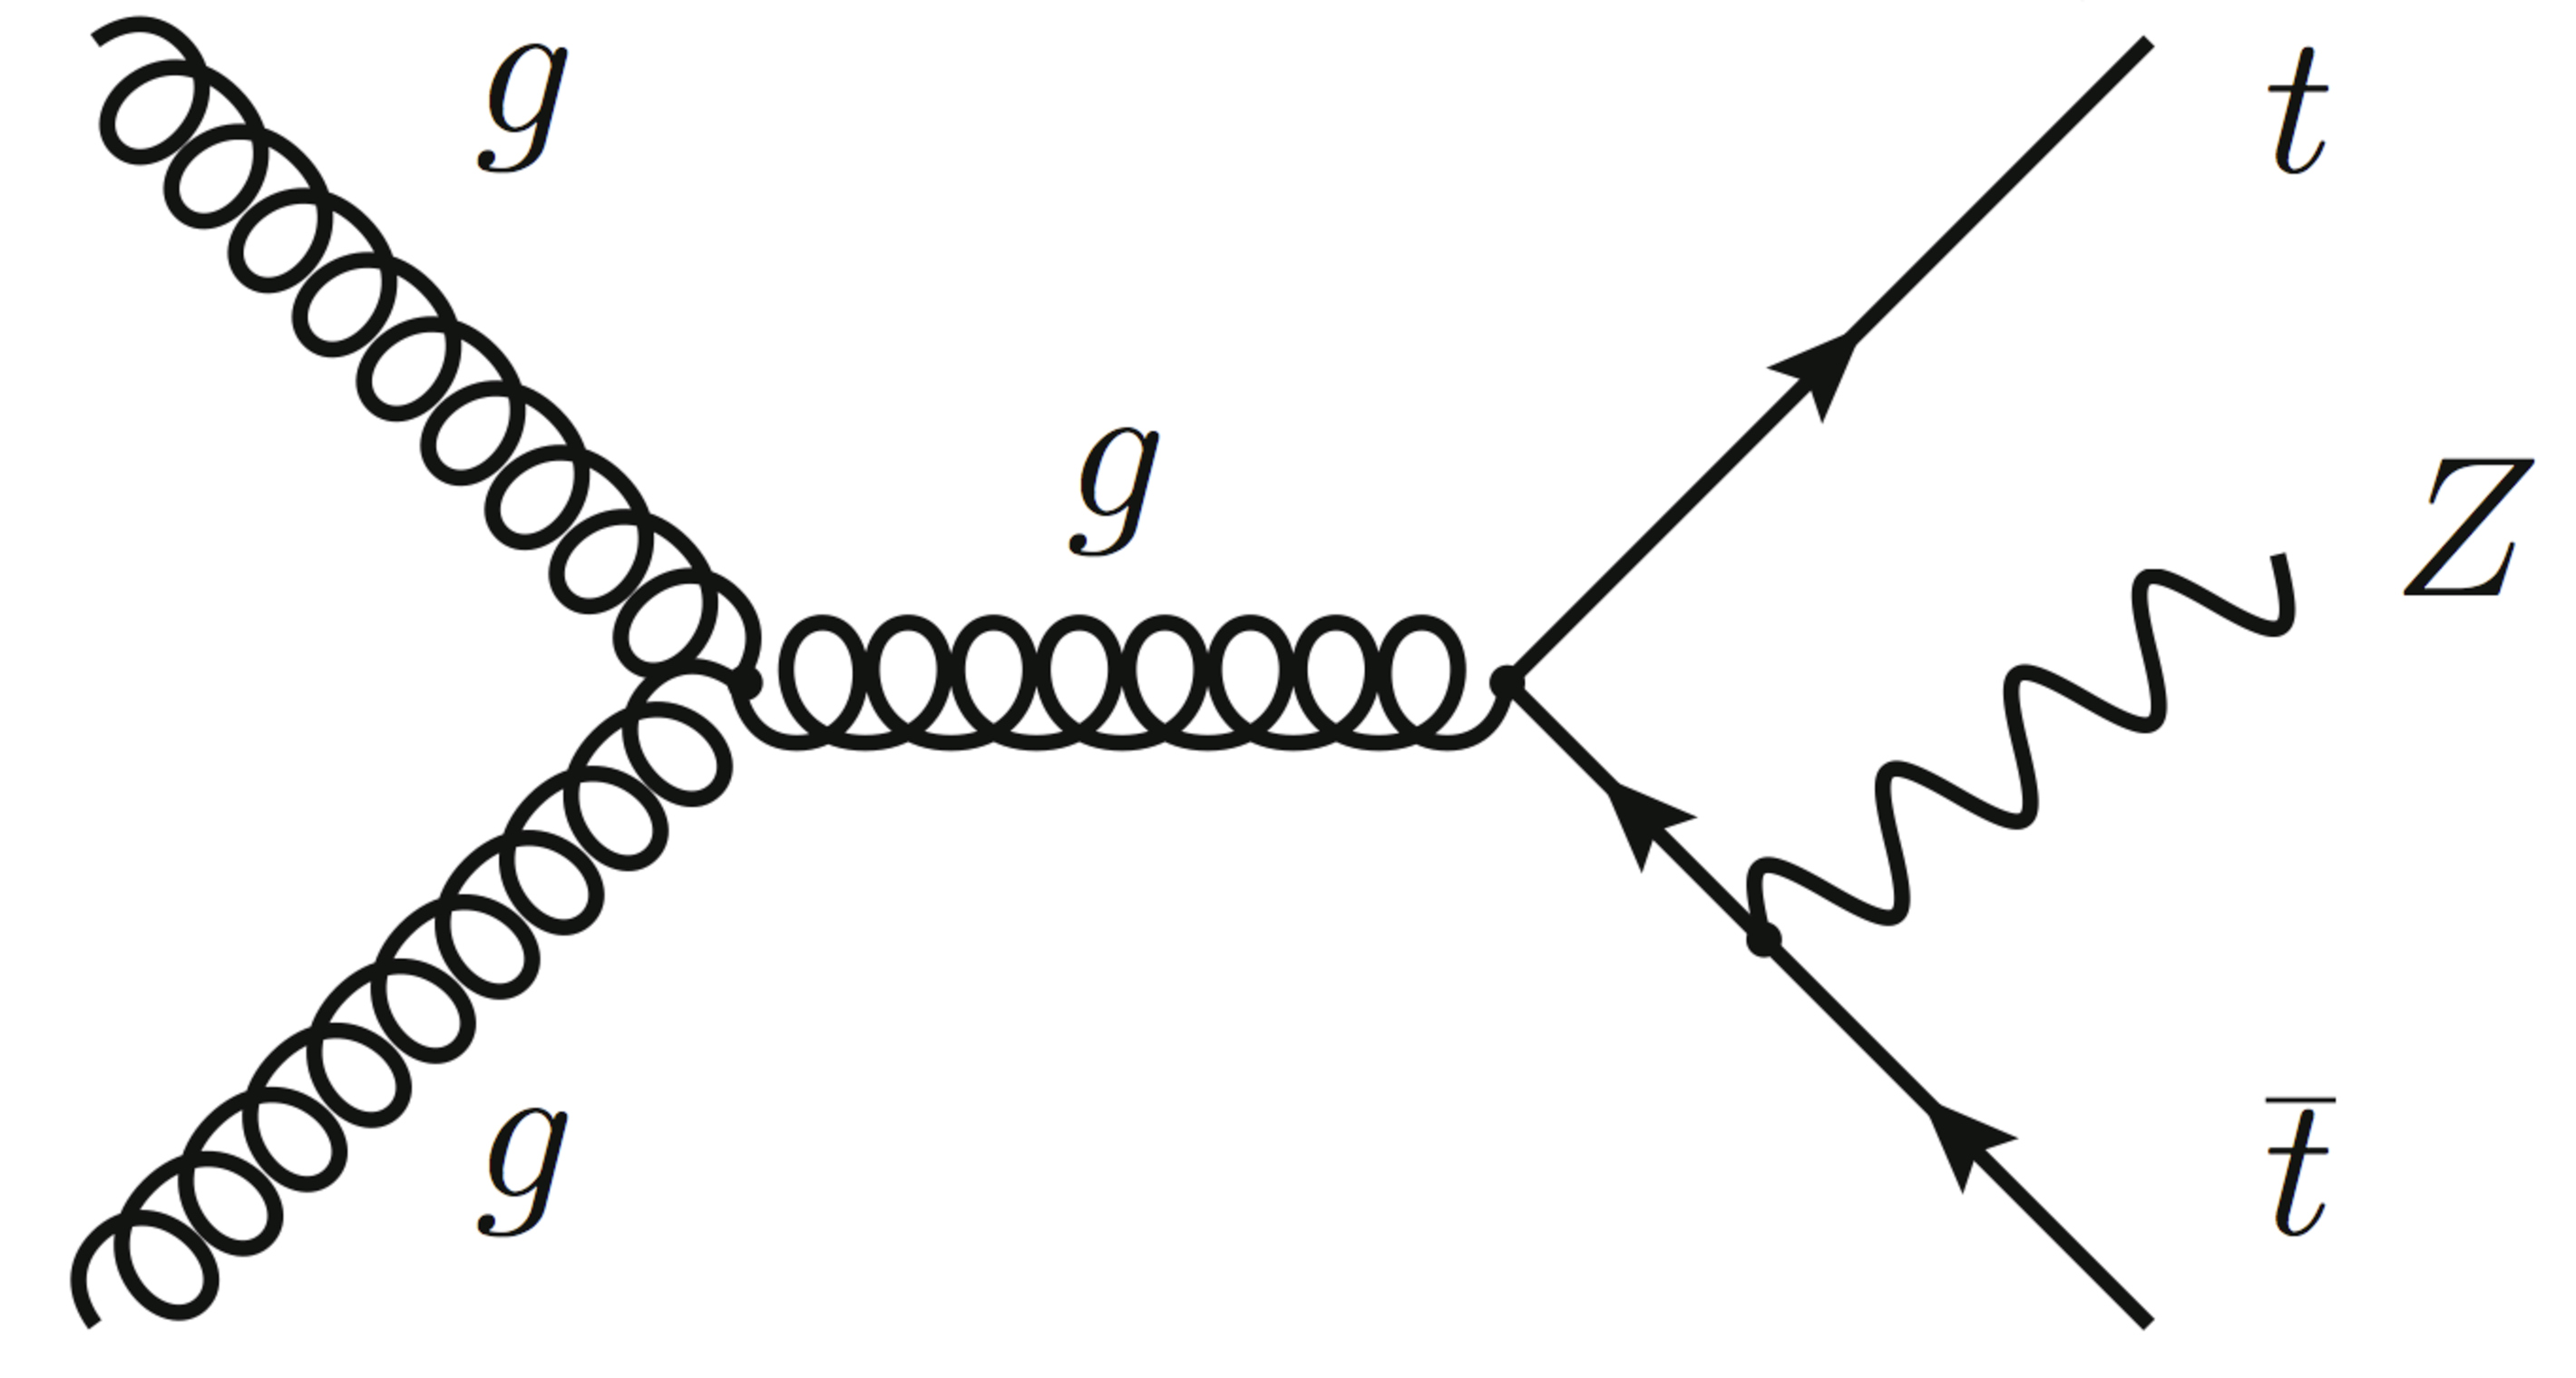
\includegraphics[scale=0.1]{ttZ_feynman.pdf}
    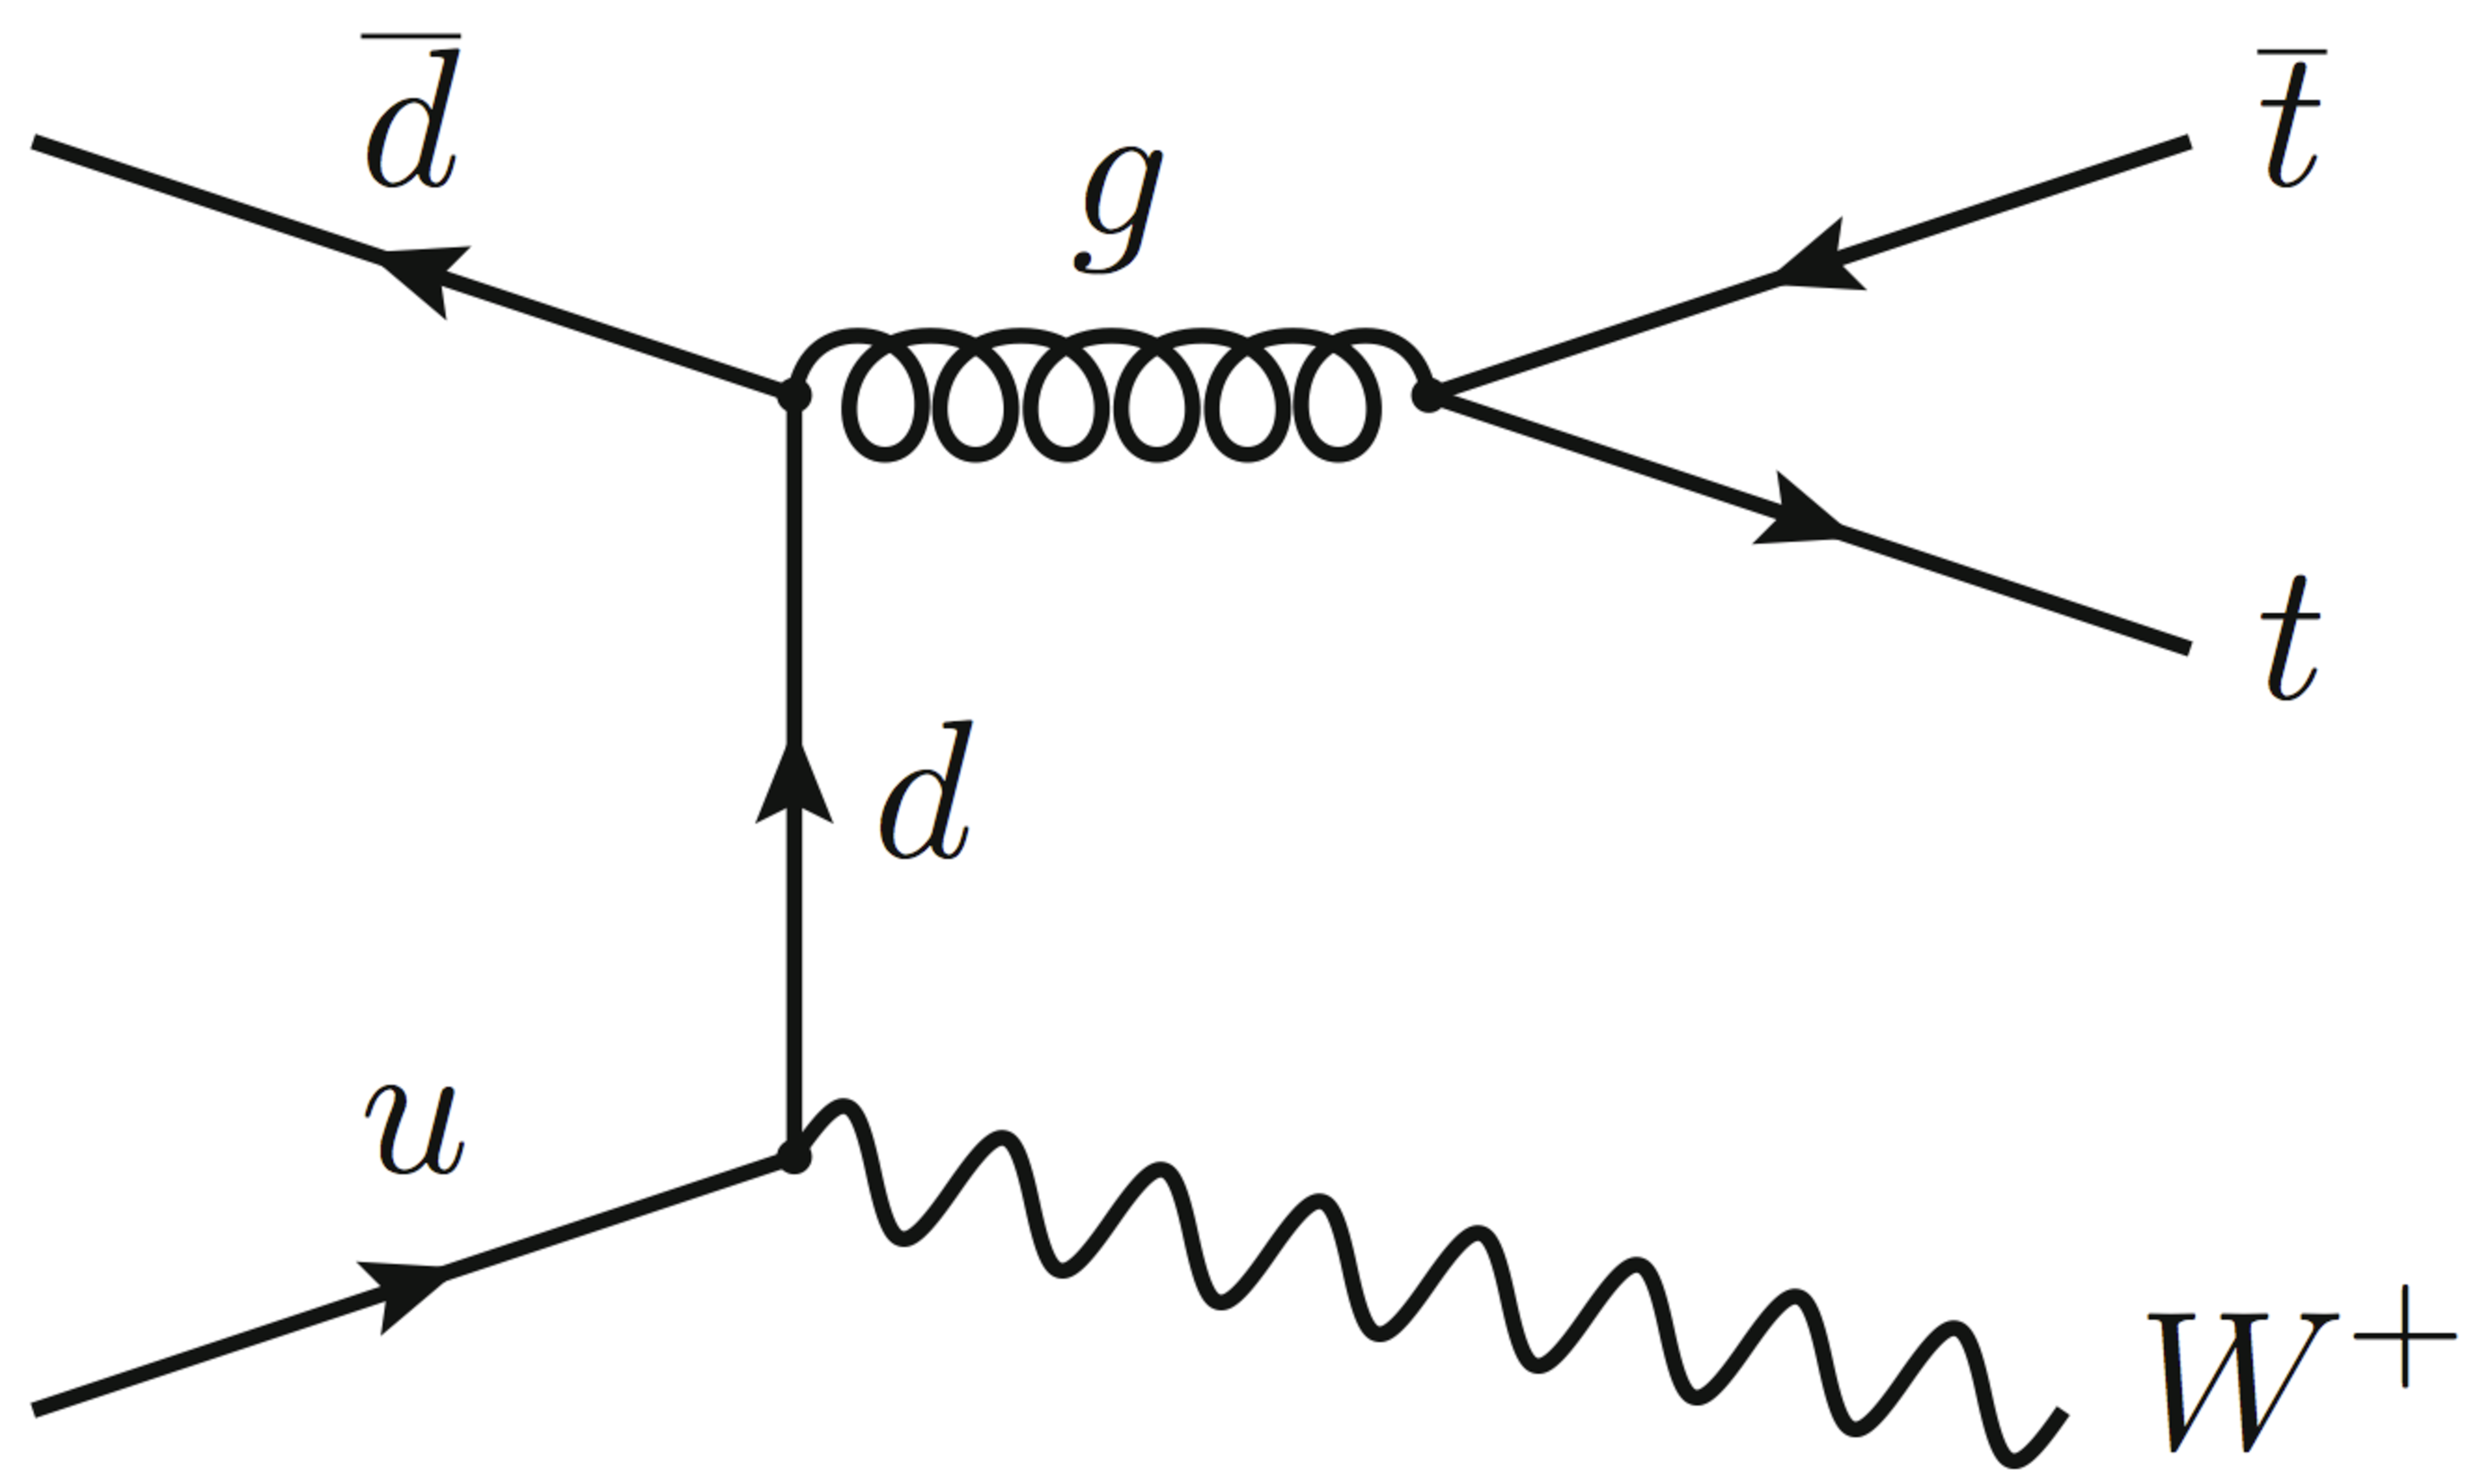
\includegraphics[scale=0.1]{ttW_feynman.pdf}
    \vspace{3mm}
    \caption{}
    \label{fig:ttV}
    % https://twiki.cern.ch/twiki/bin/view/CMSPublic/PhysicsResultsTOP14021
\end{figure}